
\def\theTopic{Helper--Hinderer }
\def\dayNum{4}


\begin{center}
\vspace*{-.2in}
{\bf {\large Helper -- Hinderer}}\\
\end{center}

Do young children know the difference between helpful and unhelpful
behavior?  A study in   {\it Nature}\footnote{ Hamlin, J. K.,
  Wynn, K., \& Bloom, P. (2007). Social evaluation by preverbal
  infants. {\it Nature}, 450, 557-559. }
reported results from a simple study of infants which was intended to
check young kids' feelings about helpful and non-helpful behavior.  

We'll watch the video of the puppet show the kids watched and see the
choice they had to make.  The research question is:
\begin{center}
  {\sf Are infants able to notice and react to helpful or hindering
    behavior observed in others?} 
\end{center}

{\bf Data}:  Of the 16 kids, 14 chose the ``helper'' toy and 2 chose
the ``hinderer''.

{\bf Discuss with your group and fill in:	}\vspace{-.3cm}
\begin{enumerate}
  \item  What proportion of the infants chose the helper toy? Include
    the correct notation. ($p$ for a population proportion, or
    $\widehat{p}$ for the sample proportion.)
\begin{students}
     \vspace{1cm}
\end{students}

\begin{key}
     {\it  $\widehat{p} = 14/16 = 0.875$ }
\end{key}
\item  
     Suppose the infants really had no preference for one toy or the other,
     and the puppet show had no effect.  What sort of results
     (numbers) would     you expect to see?
\begin{students}
       \vspace{1cm}
\end{students}

\begin{key}
       {\it  Close to 1/2 picking the helper.}
\end{key}

   \item Think back to our ``Fraud Detection'' activity on the first day of
     class.  What sort of evidence made us think the instructor really
     could distinguish coin flip sequences from made up sequences?  Note:
     it depended not just on one answer from the instructor, but also
     on the ``background'' distribution from the whole class.
\begin{students}
  \vspace{2cm}
\end{students}

\begin{key}
       {\it   We saw that relative to the class, the instructor's number
         correct was quite high.}
\end{key}
 
   \item How could you use coin flips to model a child's choice of
     toy? For 16 kids?
\begin{students}
  \vspace{2cm}
\end{students}

\begin{key}
       {\it  For one kid, let Heads = ``Helper'', tails =
         ``Hinderer''.  Count the proportion of heads in 16 flips of a
         fair coin.} 
\end{key}
   \item In using the coin, what assumption are you making about the
     kids' preferences? 
\begin{students}
  \vspace*{2cm}
\end{students}

\begin{key}
       {\it   That they are just picking one toy at random with no
         real preference for the helper or hinderer.}
\end{key}

   \item In statistical language the idea of ``no preference'' is
     called the {\bf null hypothesis}  and it is written in terms of
     the population proportion, $p=$ the true proportion of infants
     which chose the helper toy, as
      $$ H_0:\ p = 0.5.$$
     We also have an {\bf alternative hypothesis}, labeled $H_a$,
     which tells us the direction the researchers would like to
     conclude is true.  For this situation, they think there might be
     a preference toward the helper, so they would like to conclude
     that $H_0$ is wrong, and that really 
       $$H_a: \ p > 0.5 \mbox{ is true.}$$

     Under $H_0$,  is it possible that 14 out of 16
      infants could have chosen the helper toy just by chance? 
\begin{students}
  \vspace{1cm}
\end{students}

\begin{key}
{\it Yes, it is possible to get 14 or more heads. Anything is
  possible in a random sequence, but it is not very likely. }
\end{key}

\item If infants had no real preference, would the observed result (14
  of 16 choosing the helper) be very surprising or somewhat
  surprising, or not so surprising? How strong do you believe the
  evidence is against the null hypothesis?
\begin{students}
  \vspace{2cm}
\end{students}

\begin{key}
{\it Pretty surprising, strong evidence against the null.}
\end{key}

%% Use a spinner here?

  \item         {\bf Carry Out the Simulation}\\
     If you'd like to see that happen, use the
       \url{http://shiny.math.montana.edu/jimrc/spin/} Spinner web app. Set
        number of categories to \fbox{2}, labels to \fbox{hlp,hnd},
        Percentages to \fbox{50,50}, Stop after \fbox{Fixed number of
          spins}, Stop after \fbox{16} spins, and click \fbox{Run} to
        see a simulation of 16 kids choosing helper or hinderer when
        the two are equally likely. 
\begin{students}
  \vspace{1.5cm}
\end{students}

\begin{key}
{\it 12 in my first, 8 in my second }
\end{key}

    \item  Set  \fbox{1000} trials, Run, and   
              sketch your plot of 1000 trial results. 
\begin{students}
  \vspace{4cm}
\end{students}

\begin{key}
    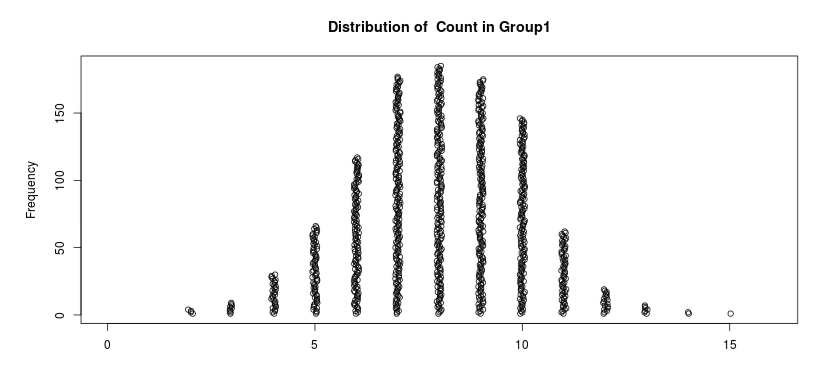
\includegraphics[width=.8\linewidth]{../plots/Helper16.png}
\end{key}
\item To see how unusual it is to get 14 or more ``helpers'' add the
  counts (for 14, 15, 16) in the table below the plot.
   How many of yours are this extreme? Circle
  these dots on your plot above. Check with the other groups
  nearby. Do we all agree?
\begin{students}
  \vspace{1.5cm}
\end{students}

\begin{key}
{\it  AWV, typically zero to 5.
}
\end{key}
\item  Do you think that babies are just blindly grabbing one of
      the toys? Explain.
\begin{students}
  \vspace{2.5cm}
\end{students}

\begin{key}
  {\it No, because it is unlikely that the observed result will pop up
    if  kids are really picking at random. }
\end{key}

  \end{enumerate}
\begin{center}
        {\large\bf Strength of Evidence}
 \end{center}
      The observed result gets compared to the distribution from the
      simulation to gauge the evidence against $H_0$.  That's
      how the scientific method works.  We formulate a hypothesis
      which can be falsified, then see if the data collected argue
      against the hypothesis. Sometimes our result provides a lot of
      evidence against the null model  -- when the observed result is very
      unlikely -- while other times it has very little evidence against
      the null model -- when the observed result is likely under the null
      model. To explain to others  how likely or unlikely the
      observed result is under the null model, we  report the
      ``strength of evidence'' -- also called the {\bf p-value}. 

      The strength of evidence is quantified by answering the
      question: ``If $H_0$ is true, what proportion of the simulated
      results are as unusual as (or even more unusual than) the
      observed result?'' 
      For example, consider the results from ``Fraud Detection''  in
      Figure 1. This instructor got 9 correct out of 12.  The
      simulation assumed $H_0: p = 0.5$, and counted the number of
      heads in 12 flips of a fair coin. (One head represents correctly
      identifying which of two sequences was generated by coin flips.)
      The whole process was simulated 1000 times and the number of
      outcomes at 9 or above on the plot are those as extreme or more
      extreme as the instructor's score. The chance is 74/1000 =
      0.074 of getting a result this extreme when $H_0$ is
      true.  We can think of 0.074 as the strength of evidence against
      $H_0$  for 9 correct matches. It is
      the probability of obtaining results as extreme or more extreme
      when $H_0$ true.
 \begin{figure}[h]
   \centering
  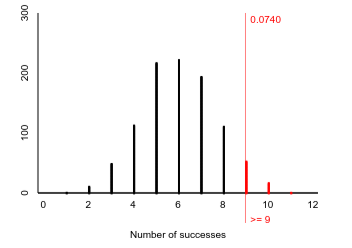
\includegraphics[width=.5\linewidth]{../plots/StrOfEvidence-12Guesses.png}

   \caption{ Simulation results obtained from the null model. The
      outcomes 9 and higher (74 out of 1000 trials) were as or more extreme
      as one instructor's number correct and indicate the strength of
      evidence of 0.074. }
   \label{fig:SOE-12}
 \end{figure}


 To help interpret strength of evidence, we offer this picture:
 \begin{figure}[h]
   \centering
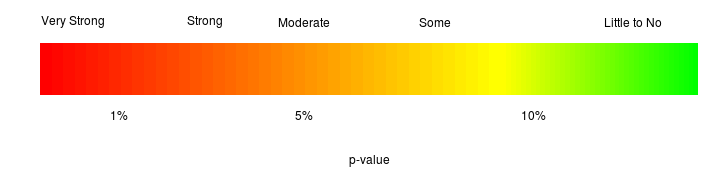
\includegraphics[width=\linewidth]{../plots/pvalueStrengths.png}
   \caption{Numeric p--value and strength of evidence}
   \label{fig:SOE-pvalue}
 \end{figure}

  The important point is that {\bf smaller} p--values (in red) provide {\bf
    stronger} evidence against $H_0$. 

  For this instructor, we would say that there is some evidence that
  they can detect fraud, but it is not super strong because a p-value
  of 0.07 is not really small.

\begin{enumerate}
  \setcounter{enumi}{11}

    \item  Use your plot from above to quantify the strength of
      evidence for the observed result 
      of 14 out of 16 infants choosing the helper toy. Give the
      numeric p--value  and a verbal description of the evidence it provides.
\begin{students}
  \vspace{1.5cm}
\end{students}

\begin{key}
{\it  1/1000 on my simulation which is ``Very Strong'' evidence
  against $H_0$.}
\end{key}

\item  What does this suggest about infants making their
      selections based only on random chance?
\begin{students}
  \vspace{4cm}
\end{students}

\begin{key}
{\it It suggests they do not make their choices based on random
 chance and do make decisions based on social interactions. }
\end{key}
\item  Put the following steps into their proper order:
 \begin{enumerate}
      \item  gather data 
\begin{key}
        {\it  2}
\end{key}

      \item  formulate a hypothesis 
\begin{key}
{\it 1   }
\end{key}

      \item  report strength of evidence 
\begin{key}
          {\it 5}
\end{key}

      \item  simulate a distribution 
\begin{key}
        {\it  3}
\end{key}
      \item  compare observed results to the distribution 
\begin{key}
        {\it  4}
\end{key}

  \end{enumerate}\vspace{1in}
\end{enumerate}

{\bf Take Home Messages}
\begin{itemize}
  \item Setting up null and alternative hypotheses is very
    important.\\
    They should be set in the planning stages of the study, not after
    looking at the data. 
    The equals sign always goes into $H_0$, but the value we set $ = p$ is not
    always .5.  The direction of the inequality in $H_a$ must match
    the researcher's ideas -- what they would like to show. It can be
    $<$, $>$, or $\neq$.  The latter means they are looking for a
    difference in either direction.
  \item It's important to know the definition of the p--value. We
    assume $H_0$ is true to compute it.  We  use a simulation based
    on the  value for $p$  in $H_0$ to calculate the p--value.    
  \item The idea of p--value is very important in statistics. It will
    follow us all the way through the course. Stronger evidence means
    {\bf smaller} p--value.  Large p--values mean the data are not
    unusual under $H_0$.
  \item In any hypothesis test, we report p--values to the reader.  
 \item 
  In the remaining space add your own summary of the lesson. Any questions?
\end{itemize}\vfill

{\bf Assignment}
\begin{itemize}
\item Quizork 3 is posted on D2L.  Turn in as a pdf file to the D2L
  drop box.
\end{itemize}

%% Uses spinner, not IntroStatShinyApps
   % Go to:
   %     \url{http://shiny.math.montana.edu/IntroStatShinyApps} and click
   %     \fbox{One Categ.}, then ``Enter/Describe Data''.
   %      Change \fbox{Success''} to \fbox{Helper} and
   %     \fbox{Failure} to \fbox{Hinderer}.  Enter the counts for each which
   %     should add up to 16 = the number of kids tested.\\
   %     Next, go back to the ``One Categ'' menu and select ``Test''.
   %     Check that   success  and failure (helper or hinderer) are
   %     equally likely. The ``Sample from Null Hypothesis'' table shows
   %     how many Helpers came up in one random sample of 16 kids.
   %     Record that here.



